\section{Event Planning}
    \subsection{Venue}

        \begin{figure}[H]
            \centering
            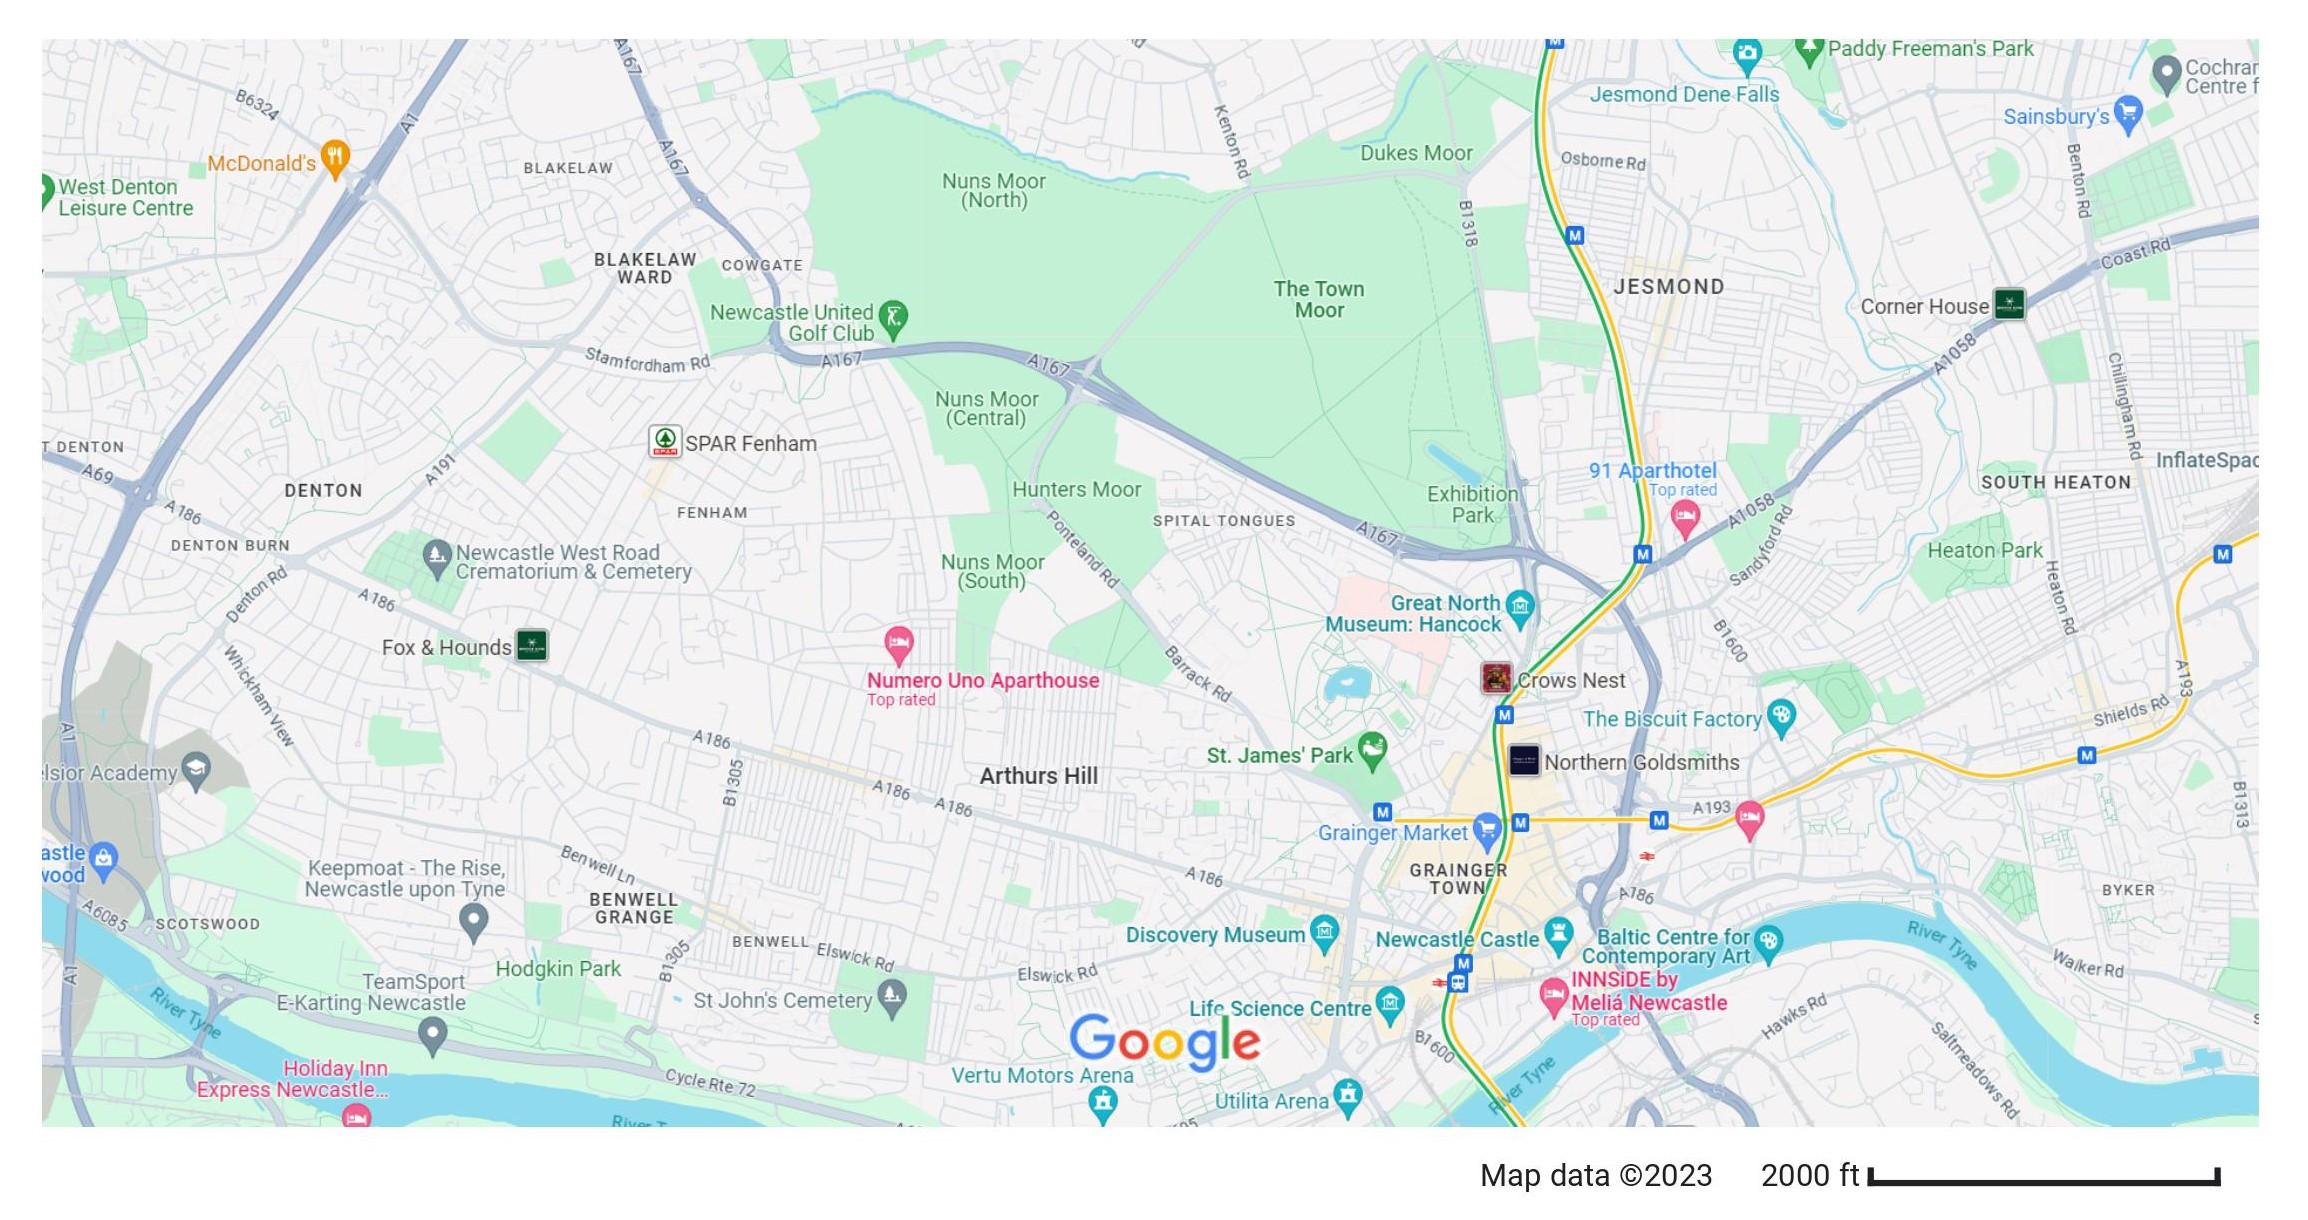
\includegraphics[width=\textwidth]{Images/festival_maps.jpg}
            \caption{Map of the surrounding area}
            \label{fig:festival_map}
        \end{figure}
        
        The Town Moor in Newcastle Upon Tyne was selected for its UK city setting, offering approximately 1,000 acres of open space to accommodate a crowd of 50,000 to 100,000 people. Situated near a well-known brewery and various amenities, this centrally located area, which has previously hosted one of Europe's largest travelling fairs, fulfils the project requirements.
        
        \begin{figure}[H]
            \centering
            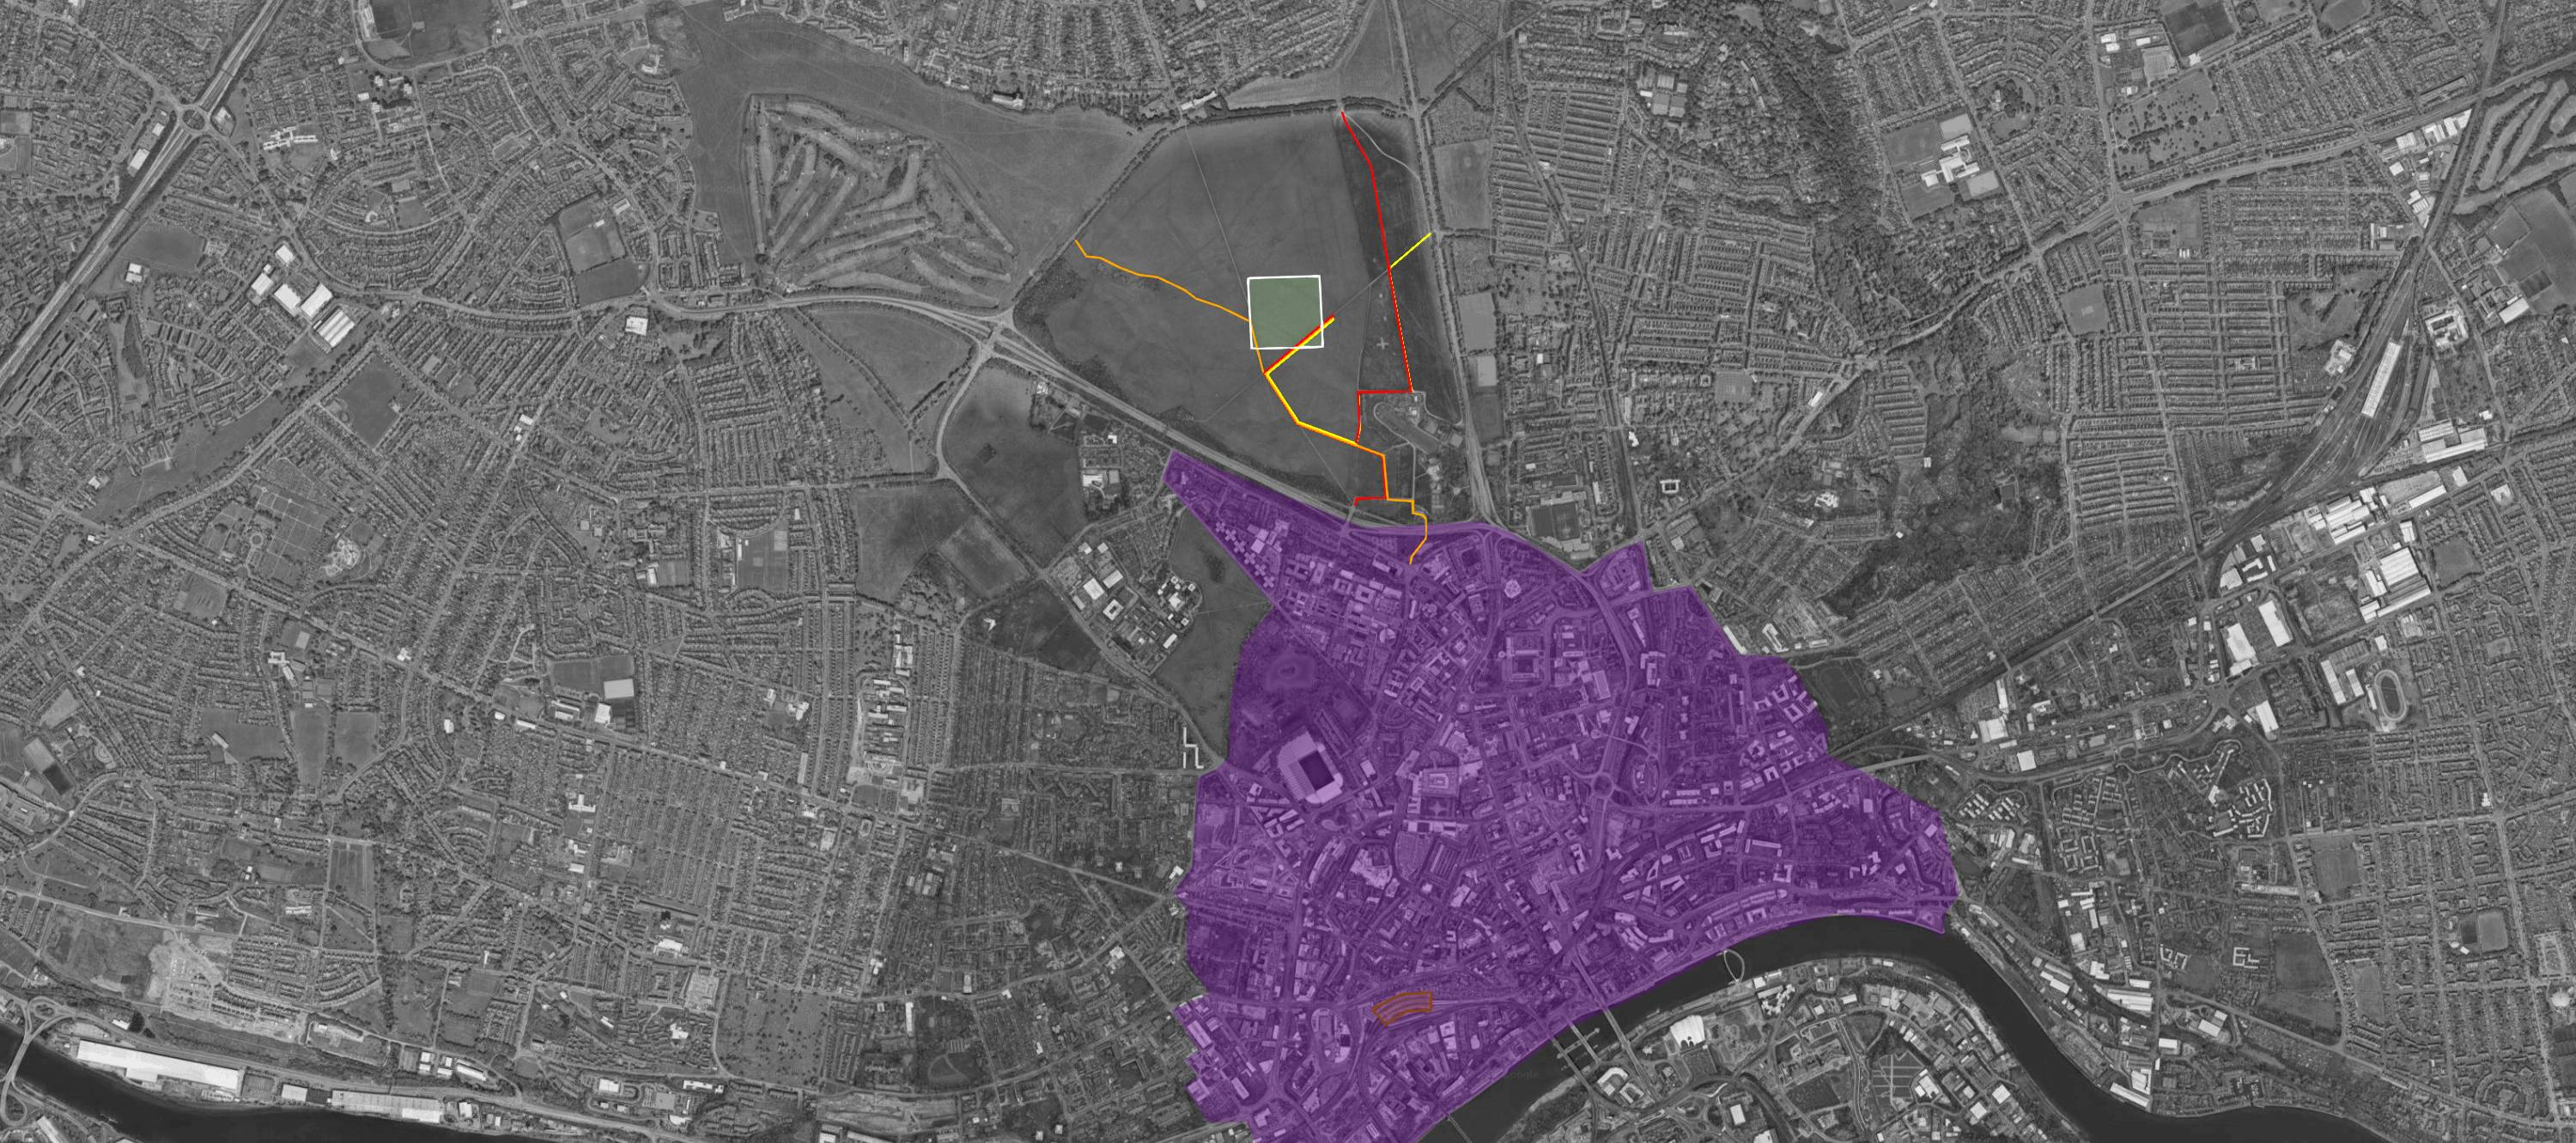
\includegraphics[width=\textwidth]{Images/festival_expand.jpg}
            \caption{Satellite image with city centre (purple), and festival location (green)}
            \label{fig:festival_expand}
        \end{figure}

        Given the proximity to busy A roads and motorways, sound pollution is anticipated to be partially masked in this area. The vast size of the park should contain most of the pollution. Strategies, including minimizing rear-firing through techniques like end-fire for a cardioid sub frequency response, will be explored. The festival's location and direction are expected to aid in dissipating audio across extended sections of the moor.
        
        \begin{figure}[H]
            \centering
            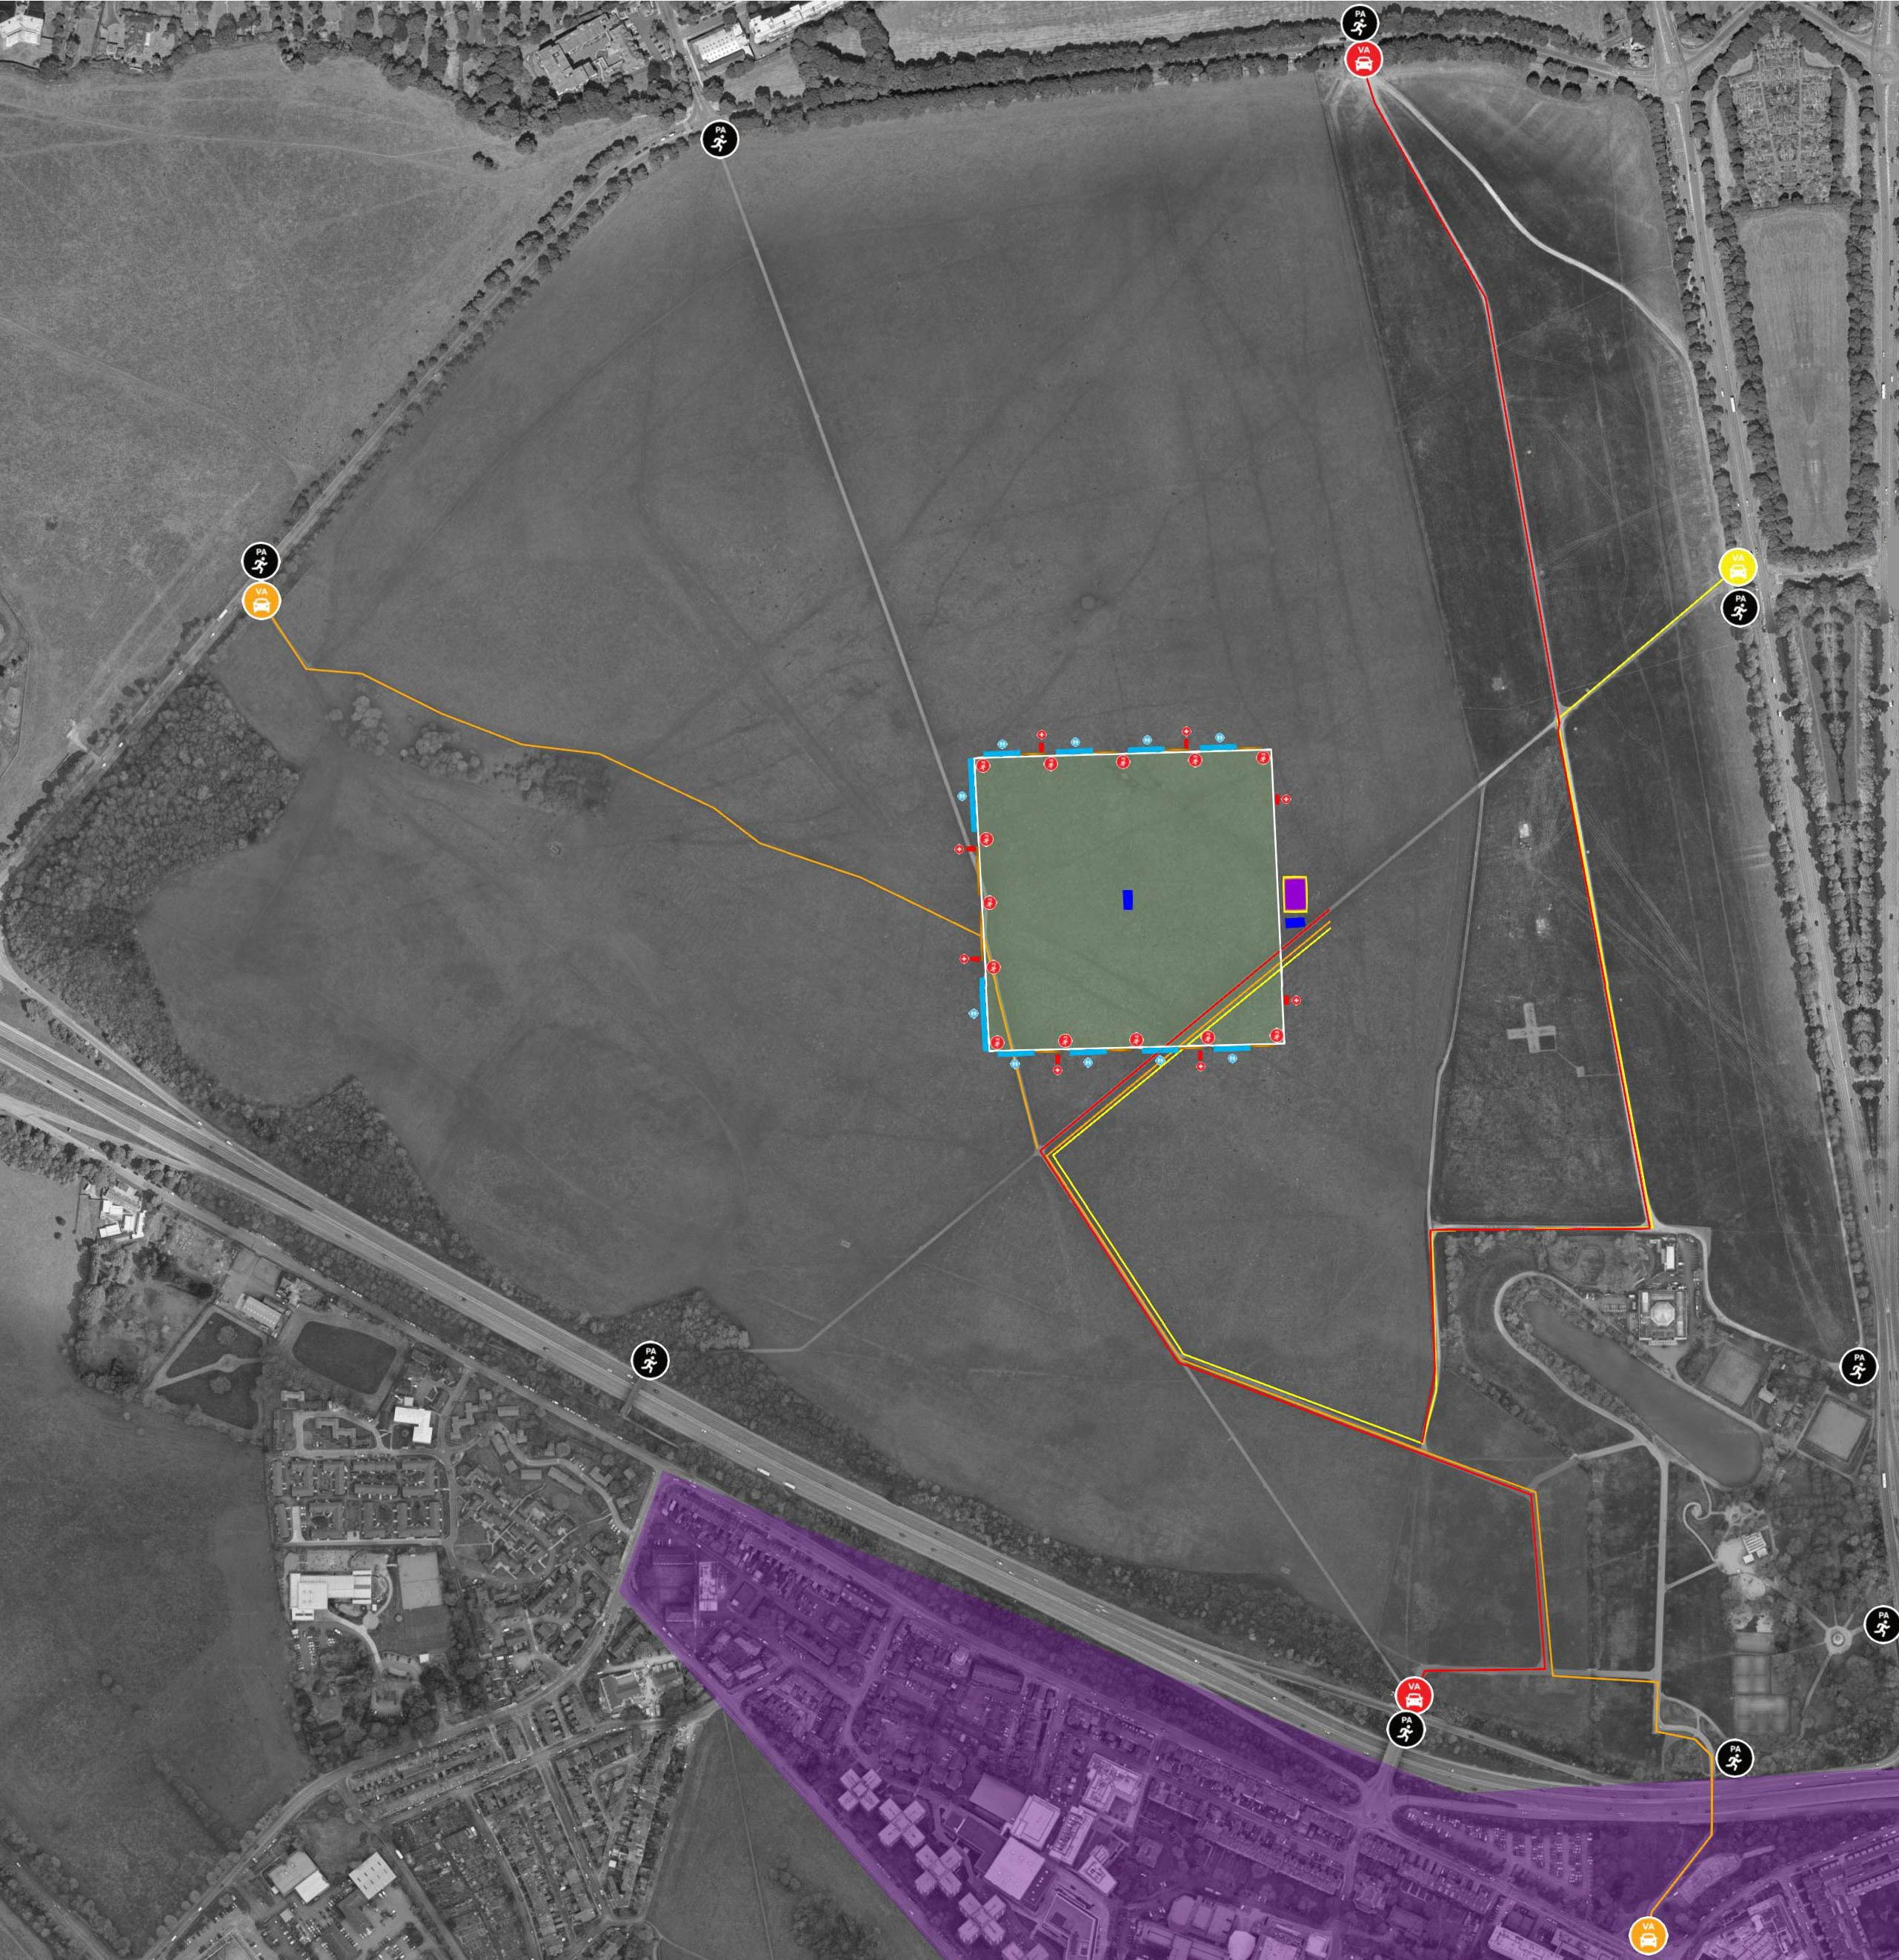
\includegraphics[width=\textwidth]{Images/festival_vap_pap.jpg}
            \caption{Festival \gls{vap} [ small (yellow) medium (orange) and large (red) ] and \gls{pap} (black)}
            \label{fig:festival_vap_pap}
        \end{figure}

        Figure \ref{fig:festival_vap_pap} shows the \gls{vap} with large, medium and small sized vehicle routes for setup and staff access. \gls{pap} indicates the access routes for pedestrians entering the festival area.

        \begin{figure}[H]
            \centering
            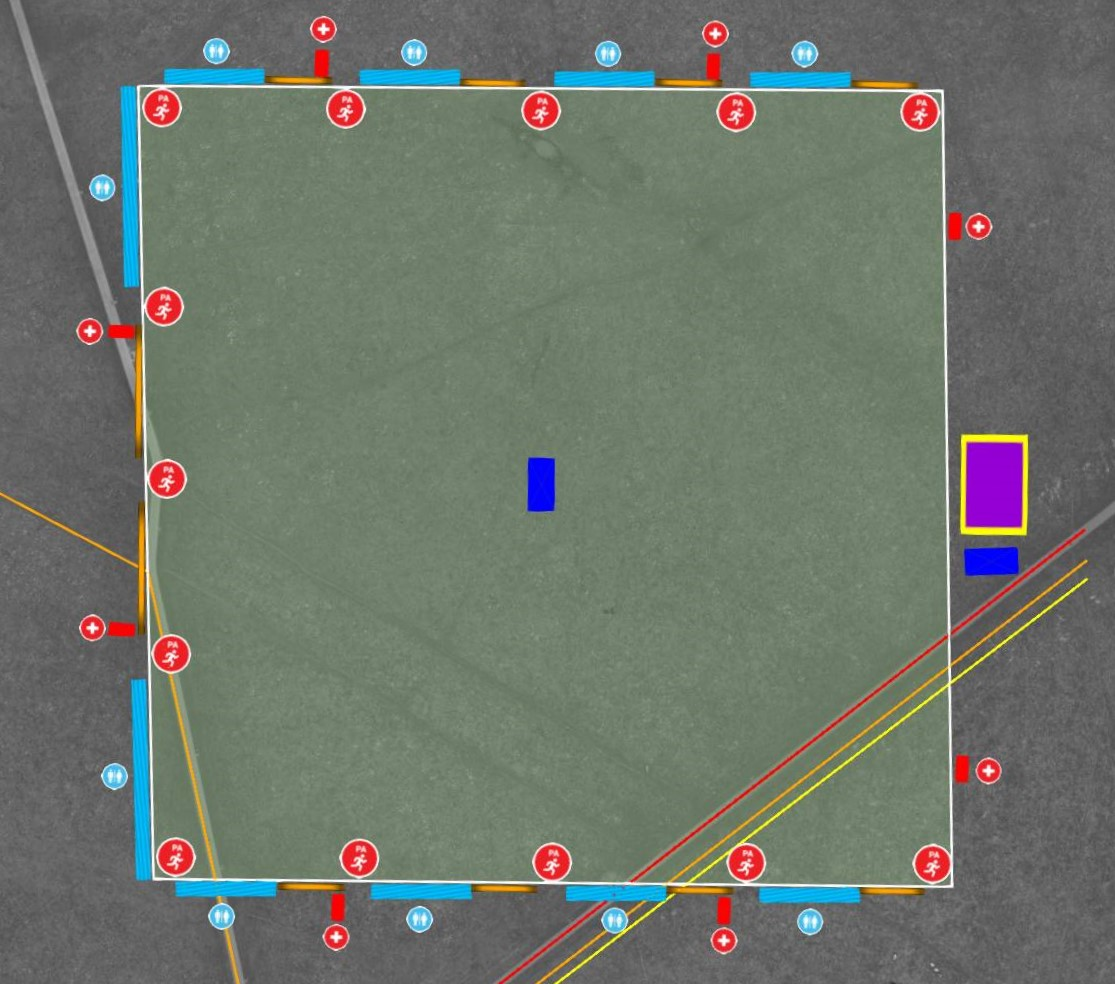
\includegraphics[width=\textwidth]{Images/festival_close_up.jpg}
            \caption{Festival layout with toilets (light blue strips), vendor booths (orange strips), medical tents (red), entrance/exit (red PA / running man), staff tents (dark blue), stage (purple)}
            \label{fig:festival_close_up}
        \end{figure}

        Figure \ref{fig:festival_close_up} shows a rough guide of various amenities, with measurements calculated as shown in Table \ref{tab:amenities_calcs} (some measurements have been rounded up for simplicity in calculations and to give room for error).

        \begin{longtable}{|p{1.5cm}|p{14cm}|}
            \hline
            \textbf{Item} & \textbf{Calculations} \\
            \hline
            \endhead % header for subsequent pages
            Total Area & To comply with fire and safety regulations, the festival's total area must be carefully allocated. According to \citet{mmontgomery2018}, the following considerations should be taken into account:
        
            \begin{itemize}
                \item At least 200 square meters must be set aside for the staging area. The requested area is $\SI{20}{\metre} \times \SI{30}{\metre}$, which equals \SI{600}{\metre\squared}.
                \item At least \SI{500}{\metre\squared} should be reserved for vendor booths, staff, security, and medical personnel. Scaling this by the same factor as the staging area, we get $3 \times \SI{500}{\metre\squared} \approx \SI{1500}{\metre\squared}$, divided into approximately \SI{500}{\metre\squared} each for vendor booths, staff \& security, and medical personnel.
                \item Under fire and health safety regulations, the remaining area should provide 2 people per square meter. For the main festival standing audience (at full capacity), an area of \SI{50000}{\metre\squared} will be required.
                \item For a moving queuing system, the guidance suggests 4 people per square meter. Therefore, an area of \SI{25000}{\metre\squared} will be allocated for the queuing audience (at full capacity).
            \end{itemize} \\
            \hline
            Exits & 
                \citet{hmgovernment2007} states that the risk of outdoor fires is typically considered lower than indoor fires due to reduced susceptibility to smoke and heat, and outdoor escape routes are less likely to be obstructed. 
    
                \textbf{Risk to Exit Time:}
                \[
                    \begin{aligned}
                          \text{High: }&   &<& \SI{5}{\minute}\\
                        \text{Normal: }& 5 &<& \SI{10}{\minute}\\
                           \text{Low: }&   &>& \SI{10}{\minute}
                    \end{aligned}
                \]
    
                \textbf{Appropriate Flow Rate for Outdoor Standing Events:}
                109 people per meter of escape width, per minute.
    
                \textbf{Total Exit Width Calculation:}
                \[
                    \text{Total Exit Width} = \frac{\text{Number of People}}{\text{Flow Rate} \times \text{Escape Time}} \approx \SI{92}{\metre}
                \]
    
                \textbf{Minimum Exit Size:}
                1.09 meters, adjustable for larger venues.
    
                To determine the required exit width for a venue, the formula considers both the nominal exits needed and an additional exit to account for potential blockages during a fire event:
                \[
                    \text{Total Exits} = \text{Nominal Exits} + 1
                \]
    
                For a given exit width of 7 meters, the nominal exits required can be calculated using the formula:
                \[
                    \begin{aligned}
                    \text{Nominal Exits} &= \frac{\text{Total Exit Width}}{\text{Exit Width per Exit}}\\
                                         &\approx 12 \text{ nominal exits}
                    \end{aligned}
                \]
    
                Additionally, the total capacity of the exits can be determined by multiplying the flow rate of 109 persons per minute by the total escape width of 92 meters:
                \[
                    \begin{aligned}
                    \text{Total Capacity} &= \text{Flow Rate} \times \text{Total Escape Width}\\
                                          &\approx 10,000 \text{ persons per minute}
                    \end{aligned}
                \]
    
                To estimate the number of people leaving within a given time frame (e.g., 10 minutes), the total capacity is further multiplied by the time:
                \[
                    \begin{aligned}
                    \text{Number of People Leaving}
                    &= \text{Total Capacity} \times \text{Time}\\
                    &\approx 100,000 \text{ people for 10 minutes}
                    \end{aligned}
                \]
    
                Therefore, a total of 13 exits with a width of 7 meters will be required.
            \\
            \hline
            Vendor Booths &
                According to information from \citet{jjones2023}, food trucks are typically \SI{5}{\metre} long by \SI{2}{\metre} wide, but can range from \SI{3}{\metre} to \SI{8}{\metre} long by \SI{2}{\metre} to \SI{3}{\metre} wide. Let's assume we have $\SI{5}{\metre} \times \SI{2}{\metre}$ trucks, which equals \SI{10}{\metre\squared}. With the available area of \SI{500}{\metre\squared}, we can accommodate 50 vendor booths $(\SI{500}{\metre\squared} \div \SI{10}{\metre\squared})$.
            \\
            \hline
            Medical Regulations &
                Based on first aid cover guidelines from \citet{sja2023} and ambulance size specifications from \citet{nhs-ambulance-specs}, the medical regulations can be calculated as follows:

                First aid cover:
                \begin{itemize}
                    \item 2 first aiders per 1,000 people = 200 first aiders
                    \begin{itemize}
                        \item 152 first aiders in and around the crowd
                        \item 48 in tents (6 per tent for 8 tents)
                    \end{itemize}
                    \item Standard first aid tent size = $\SI{8}{\metre} \times \SI{4}{\metre} = \SI{32}{\metre\squared}$
                \end{itemize}

                Ambulance size = $\SI{2.45}{metre} \times \SI{6.95}{\metre} \approx \SI{18}{\metre\squared}$.

                According to \citet{hmas-festivals}, for festivals with 4,000 people, 1 ambulance or response vehicle is recommended, therefore 100,000 people require 25 ambulances or response vehicles.
            \\
            \hline
            Toilets &
                For a large music events featuring alcohol, food, and drinks, the required toilets can be calculated using the following guidelines from \citet{lsharp2023} and \citet{andyloos2015}:

                \begin{itemize}
                    \item Women: 1 portaloo per 75 people
                    \item Men: 1 portaloo per 400 people
                    \item Men: 1 urinal per 100 people
                \end{itemize}
                
                Taking into account the percentage split of men to women at festivals (e.g., at Latitude Festival, the split was 40\% women and 60\% men \citep{aawbi2019}), therefore, considering an example with 100,000 attendees, the minimum required toilets would be:
                
                \begin{itemize}
                    \item Total minimum: 1000
                    \item Women's toilets: 534
                    \item Men's toilets: 150
                    \item Urinals: 600
                \end{itemize}
                
                Therefore, based on standard portaloo sizes of $\SI{1.1}{\metre} \times \SI{1.2}{\metre}$, arranged in rows of 42 toilets per row, with pairs of rows back to back, this requires 12 pairs of rows. Taking up a total of \SI{1320}{\metre\squared}:

                \[
                    \begin{aligned}
                    \SI{1.1}{\metre} \times \SI{1.2}{\metre} &= \SI{1.32}{\metre\squared} &\text{ for 1 portaloo}\\
                    \SI{1.32}{\metre\squared} \times 1000 &= \SI{1320}{\metre\squared} &\text{ for 1000 portaloos}
                    \end{aligned}
                \]
            \\
            \hline
            \gls{foh} and Backstage Areas &
                Tents with the dimensions of $\SI{20}{\metre} \times \SI{10}{\metre}$ will be provided for each: \gls{foh} ($\approx \SI{120}{\metre}$ away from stage), stage left and stage right. A backstage truck provides a $\SI{50}{\metre} \times \SI{10}{\metre}$ area for artists and backline tech.
            \\
            \hline
            Security &
                Security barriers will be setup \SI{1.2}{\metre} high, with a minimum of \SI{1.8}{\metre} from the stage, running entire length of the stage and wings. A non-transparent barricade will be erected to isolate back stage areas from audience. A Mojo barrier will be place around the \gls{foh} location within the audience. \citet{westminster2023} suggests 1 security staff to every 100 attendees will be required, totalling 1,000 staff for the event.
            \\
            \hline

            \caption{Calculation of all amenities}
            \label{tab:amenities_calcs}
        \end{longtable}

    \subsection{Regulations and Guidance}
        During indoor rock concerts, sound levels typically surpass 100 dBs for extended periods, with peaks reaching 130 dB. However, there's limited data on sound exposure at outdoor music festivals, particularly those spanning multiple stages across several days \citep{rmbrecht2023}.

        As the LAeq will exceed \SI{96}{\dB}, tickets, advertising and notices at entry points will advise the audience of the risk to their hearing in advance \citep{hse-event-safety-noise}. Hearing protection will be provided to all staff and audience members on the door as The Control of Noise at Work Regulations (\citeyear{hse2005}) state that any prolonged exposure to noise of over \SI{85}{\decibel} in the workplace requires ear protection. Additionally, younger kids who may attend have sensitive hearing and anything over \SI{85}{\dB}, even for a short exposure time, can cause damage \citep{rmbrecht2023}.

        \citet{hse-event-safety-noise} states that the continuous A-weighted \gls{spl} over an event should not exceed \SI{107}{\dB} and the C-weighted peak \gls{spl} should not exceed \SI{130}{\dB} within the audience. Therefore, during soundcheck and at intervals throughout the festival, the \gls{foh} will perform regular \gls{spl} checks using a 10Easy system with Rational Acoustics's software 'Smaart'. The audience to loudspeaker separation distance should also exceed \SI{1}{\metre} to help reduce the peak levels within the area.